\normaltrue
\correctiontrue

%\UPSTIidClasse{11} % 11 sup, 12 spé
%\newcommand{\UPSTIidClasse}{12}

\exer{Mouvement T -- $\star$ \label{B2:13:01:02}}
\setcounter{numques}{0}
\UPSTIcompetence[2]{B2-13}
\index{Compétence B2-13}
\index{Mécanisme à 1 translation}
\ifcorrection
\else
\textbf{Pas de corrigé pour cet exercice.}
\fi

\ifprof
\else ~\\
Soit le mécanisme suivant. On note $\vect{AB}=\lambda(t)\vect{i_0}$.
\begin{center}
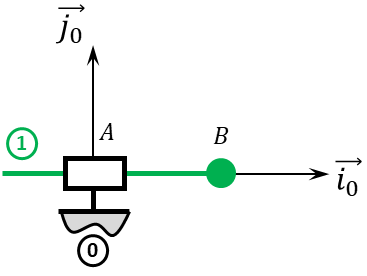
\includegraphics[width=.6\linewidth]{01_T_01}
\end{center}
\fi

\question{Donner le torseur cinématique $\torseurcin{V}{1}{0}$ au point $B$.}
\ifprof ~\\
$\torseurcin{V}{1}{0} = \torseurl{\vect{0}}{\dot{\lambda}(t)\vi{0}}{\forall P}$.

$\vectv{B}{1}{0} = \deriv{\vect{AB}}{\rep{0}}=\dot{\lambda}(t)\vi{0}$.
\else
\fi

\question{Déterminer $\vectg{B}{1}{0}$.}
\ifprof  ~\\
 $\vectg{B}{1}{0} = \deriv{\vectv{B}{1}{0}}{\rep{0}}=\ddot{\lambda}(t)\vi{0}$.
\else
\fi


\ifprof
\else
\footnotesize
\begin{center}
\begin{tabular}{|p{.9\linewidth}|}
\hline
Indications :
\begin{enumerate}
\item $\torseurcin{V}{1}{0} = \torseurl{\vect{0}}{\dot{\lambda}(t)\vi{0}}{\forall P}$.
\item  $\vectg{B}{1}{0} =\ddot{\lambda}(t)\vi{0}$.
\end{enumerate} \\ \hline
\end{tabular}
\end{center}
\normalsize

\begin{flushright}
\footnotesize{Corrigé  voir \ref{B2:13:01:02}.}
\end{flushright}%
\fi


